\section{Network Architecture}
\label{sec:architecture}

The overall architecture of the network components can be seen in
Figure~\ref{fig:network}. 
The network architecture can be divided largely into two parts, the network
layer and the transport layer. The network layer is implemented in the form of
the router, and the transport layer is implemented in the endpoints that are
chained to the router interface. Flow control is implemented in both layers.
Link level flow control is implemented in the network layer so that back
pressure can be propagated across the network to ensure there are no packet
drops. End-to-end flow control is implemented in the transport layer so packets
in the network are always assured to have empty receiving buffers.

The distributed application components communicate with remote nodes using the
network \textit{endpoints}. Endpoints expose send and receive interfaces, and
behaves like a FIFO, in that it blocks when it cannot safely send any more packets.
Many endpoints can be instantiated, resources permitting, and each
endpoint can have a different \textit{type}, meaning it can expose send and
receive interfaces of different bit widths. Sending a message can be done by
calling \textit{send} with the data and destination node ID, and \textit{receive}
returns a tuple of data and source node ID.


\begin{figure}[h]
	\begin{center}
	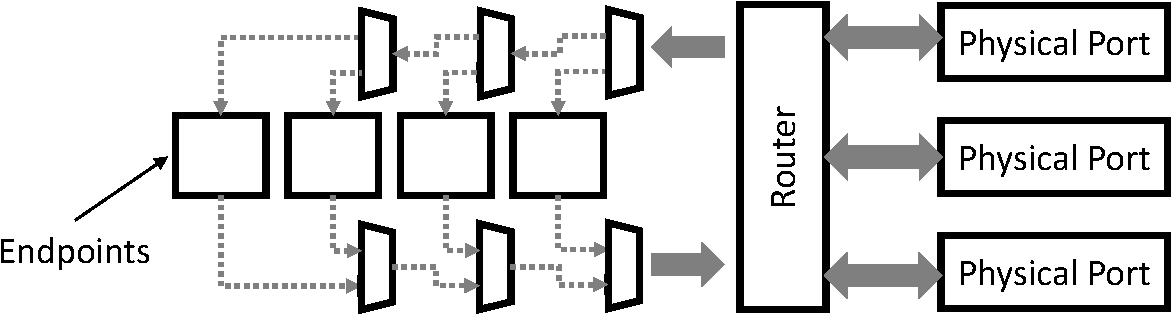
\includegraphics[width=0.45\textwidth]{resources/routing-crop.pdf}
	\caption{Network Architecture}
	\label{fig:network}
	\end{center}
\end{figure}


\subsection{Network Layer}
\label{sec:networklayer}

The network layer implements lossless, in-order routing, which assures that
packets always arrive in the order they were sent. This removes the need for
try-resend or reordering functionalities at the transport layer, allowing a much
simpler design.

\emph{\bf{Router Architecture :}}
The router logic is deterministic, in that a certain packet type from a certain
source node being delivered to a certain destination node will always travel
through the same path, even when there are multiple possible paths. Parallelism
is achieved by distributing packets from different endpoints to different paths,
when there are multiple different paths that the packet can be routed through.
This is to ensure in-order delivery of packets to an endpoint, eliminating the
need for packet reordering logic and buffer resources at the receiving end.
Because this design eliminates network level congestion control, the network may
suffer suboptimal performance if one endpoint generates the majority of network
traffic.

Each physical port implements a link-layer flow control. It has a large enough
buffer to saturate the physical link bandwidth, and assures there are no packet
drops when even the data rate exceeds to available physical bandwidth.

\emph{\bf{Endpoint Interface :}}
User endpoints expose two
separate interfaces, the user interface and the system interface. The user
interface exposes send and receive ports for the application to use to
communicate with remote nodes, while the system interface exposes another set of send
and receive ports, which are chained together to communicate with the router, as
seen in Figure~\ref{fig:network}.
The multiplexers used to chain the
endpoints together are designed to have alternating priorities between its two
inputs, in order to achieve fairness while maintaining high performance.

The system interface of each endpoint can send a pair of payload and destination
node ID to the endpoint chain. The chain logic will augment the packet with the
packet type, which is the index of the endpoint in the endpoint chain. The final
piece of the packet is the source node ID, which is filled out at the router.
The system interface can also receive a pair of payload and source node ID. The
router inserts a received packet into the endpoint chain if the destination node
ID matches its own, and the chain logic forwards the packet to the correct
endpoint according to the packet type.


\emph{\bf{Packet Structure :}}
The network layer manages packet forwarding between the user endpoints, and the
physical ports that connect to neighboring nodes. Each packet consists of four
fields: source node ID, destination node ID, packet type and payload data. The
contents of a packet can be seen in Figure~\ref{fig:packet}. Each packet is
broken into multiple fixed-width \textit{beats} when it's sent over the physical link.
The control field at the beginning is used to deliver meta-information, to
designate the beat as a flow control credit, or to mark the beat as the
last one of a packet.
The router is oblivious to the existence of multiple network endpoints or
virtual channels they represent. The router only deals with routing individual
packets, and higher level functions such as virtual channels and end-to-end flow
control is implemented by the chain of endpoints.

\begin{figure}[h]
	\begin{center}
	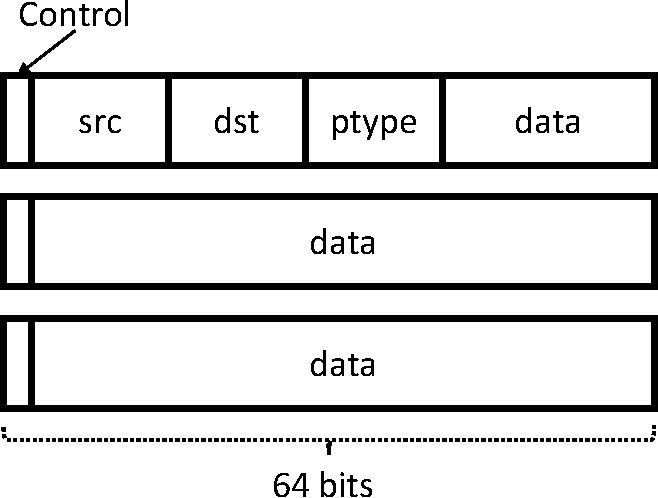
\includegraphics[scale=0.45]{resources/packet-crop.pdf}
	\caption{Packet Structure}
	\label{fig:packet}
	\end{center}
\end{figure}







\subsection{Transport Layer}
\label{sec:transportlayer}

Virtual channels multiplex a single physical network link to provide the logical
interface of multiple links. Figure~\ref{fig:virtual} describes the flow of
packets in such an environment. For virtual channels to be useful, the channels
needs to be logically separate so that they do not interfere with each other. 
Unless they are safely separated, traffic congestion in one channel can cause
the physical link to become congested and cause other channels to block. 
Our network implements a per-channel end-to-end flow control, so that a sender
can only send data onto the network when it is guaranteed that the receiving
endpoint has enough buffer space to accommodate it. This assures the physical
link and router will never deadlock, which will cause the whole network to stop.

\begin{figure}[h]
	\begin{center}
	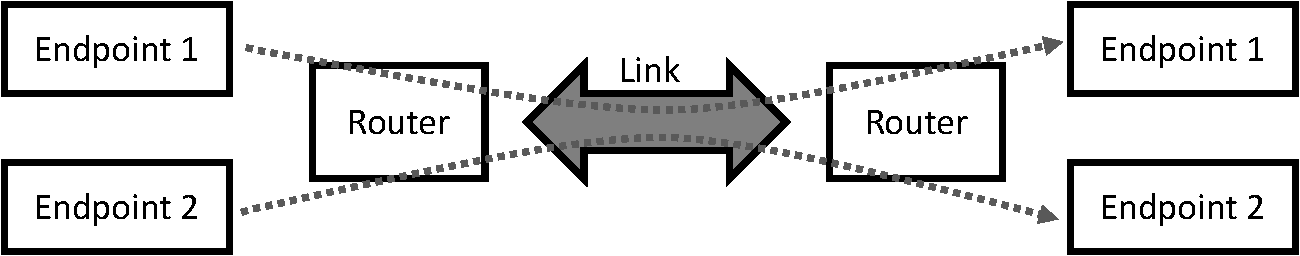
\includegraphics[width=0.45\textwidth]{resources/virtual-crop.pdf}
	\caption{Packet Flow in Virtual Channels}
	\label{fig:virtual}
	\end{center}
\end{figure}


The transport layer is implemented in individual endpoints, and its design aims
to provide a very low latency and efficient memory space usage. Each design can
have multiple instantiations of endpoints, parameterized differently. Each
endpoint act as a virtual channel entry and exit points.
The structure of an endpoint is described in Figure~\ref{fig:endpoint}. An
endpoint performs two major functions: Managing packet transfer between the user
application logic and the router layer, and end-to-end flow control. The network
also provides an unmanaged endpoint, which does not provide flow
control guarantees but provides fastest performance.


\emph{\bf{Packet Management :}}
Packets
arriving from end endpoint chain are enqueued into the receive buffer as tuples
of source node ID and packet data, and the user logic can dequeue the receive
buffer to consume the packet. User logic can send a packet to a virtual channel
by inserting a tuple of destination node ID and packet data into the send
buffer. Independently from this, the endpoint internal logic can insert flow
control packets into the ack queue to notify remote endpoints of available
buffer space, and a multiplexer interleaves packets from the send buffer and ack
queue onto the endpoint chain. When a packet arrives from the endpoint chain
that is directed at this particular endpoint, it is pushed into the receive
queue. The flow control logic ensures there is always available space in the
receive queue, and the user logic can receive a pair of source node ID and
payload data by dequeuing from the receive queue.


\begin{figure}[h]
	\begin{center}
	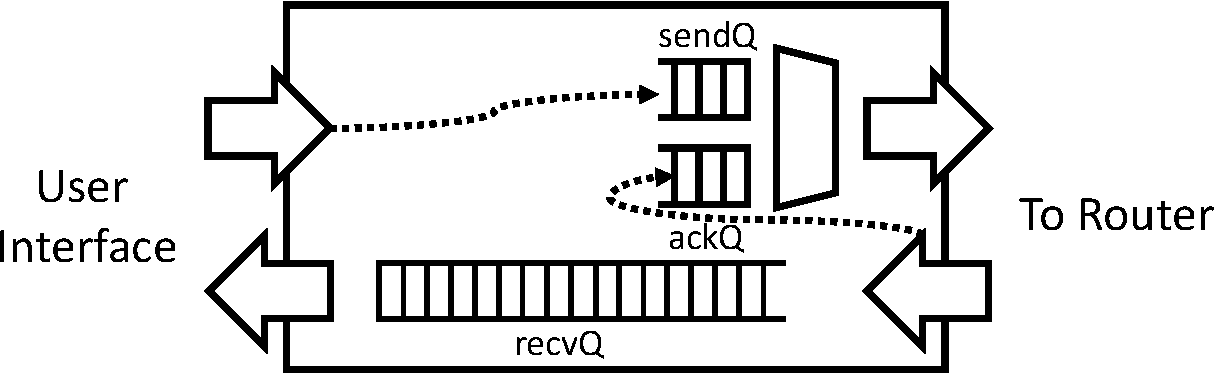
\includegraphics[width=0.45\textwidth]{resources/endpoint-crop.pdf}
	\caption{Endpoint Architecture}
	\label{fig:endpoint}
	\end{center}
\end{figure}

\emph{\bf{Parameterized Flow Control :}}
Whenever a packet is received by an endpoint, it checks a table of packets
received per source node to determine if it is time to send a flow control
credit to the source node. If the send budget of the source node is predicted to
have become small enough, it enters a request into the ack queue. A
multiplexer that arbitrates the send and ack queues only sends the flow control
packet into the network if there is enough space left on the receive buffer, and
then marks an amount of space as allocated. By enqueuing flow control packets
and sending them as soon as buffer space is ready, the sender can receive send
budget updates at a low latency without having to repeatedly send requests.

Determining when is the right time to send a flow control packet is very
important in an effective endpoint design.
In order to maintain a high bandwidth, the data
transfer packets and flow control packets must be overlapped, as seen in the
different between Figure~\ref{fig:packettiming} (a) and
Figure~\ref{fig:packettiming} (b). For such an overlap to happen, the flow
control packet must be sent a certain amount of time before the send budget of
the source node runs out. Ideally, the space allocated per flow control packet
(or \texttt{Stride})
is large enough, and the packet send offset large enough, that the flow control
packet will receive it before its budget runs out. However, it is often not
possible to provide a large enough buffer to conservatively accommodate traffic
from all nodes in the system.

\begin{figure}[h]
	\begin{center}
	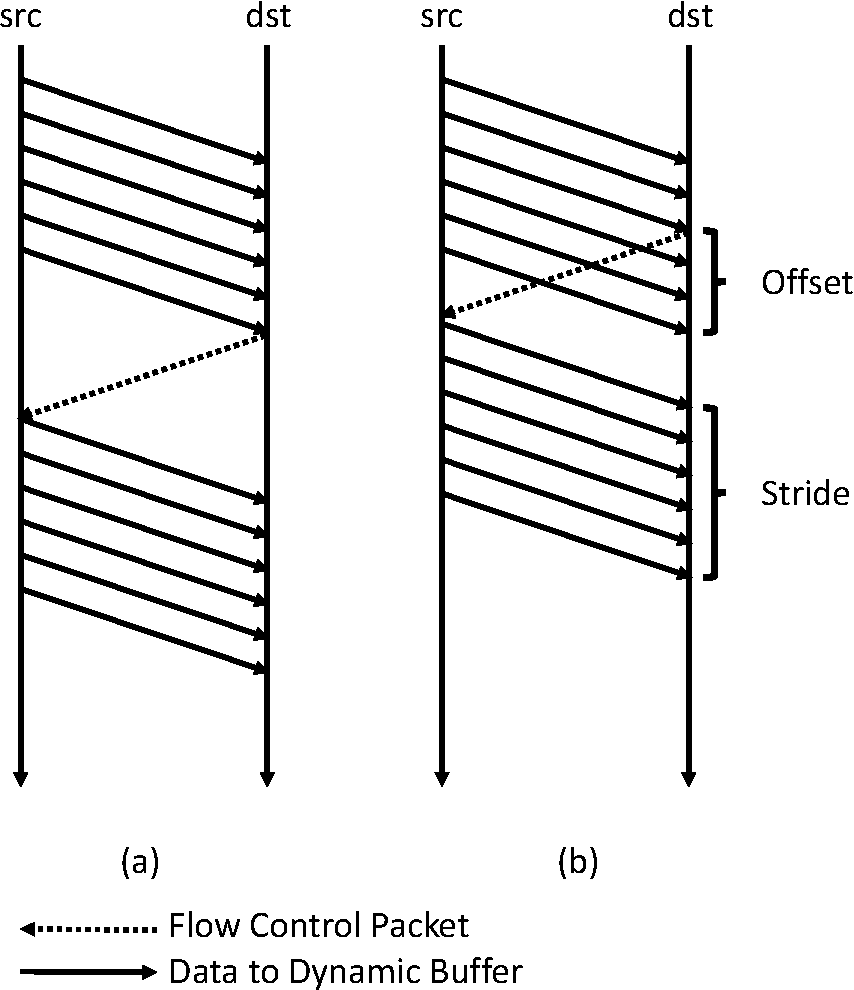
\includegraphics[width=0.25\textwidth]{resources/packettiming-crop.pdf}
	\caption{Packet Timing Comparison}
	\label{fig:packettiming}
	\end{center}
\end{figure}

Under such constraints, each endpoint can have a different flow control
configuration that attempts to best suit its usage. For example, for some endpoints
the expected traffic pattern may be that most of the data transfer happens
between a pair of two nodes. In such a case, it might be effective to have a
very low granularity flow control (or a large \texttt{Stride}), so that a large
buffer is allocated on request, but the total receive buffer may be small. On
the other hand, if many nodes are expected to send data to one node, a fine
granularity (or smaller \texttt{Stride}) flow control and a large buffer may be
required for performance. If the endpoint is used for low-bandwidth traffic such
as commands, the buffer size and granularity can be set to a small value.  To
enable such control, endpoints are initialized with the parameters described in
Table~\ref{tab:transportparamter}.

\begin{table}[b]
	\begin{tabular}{l | l}
		Parameter & Description \\
		\hline
		BufferSize & Size of the total allocated buffer space\\
		FlowOffset & Offset of flow control packet transmission\\
		FlowStride & Number of packets each flow control credit represents\\
		\hline
	\end{tabular}
	\caption{Endpoint Parameters}
	\label{tab:transportparamter}
\end{table}

Initially, all nodes start with a small send budget (\texttt{initBudget}) to all
remote nodes, and therefore the actual size of the receive packet buffer is
$initBudget \times nodeCount$ slots larger than the \texttt{BufferSize}
parameter. When the first packet arrives, space in the receive buffer is
allocated to the source node and a flow control packet is sent. When a node
decides it will not send more packets for some time and will rather stop
receiving flow control packets, it can set a bit in the packet control field
that tells the receiving endpoint to only allocate \texttt{initBudget} for the
next stride, so the send budget state can go back to its initial state. Yielding
buffers like this achieves better buffer usage when many nodes are going to send
data to one node. The receiving endpoint can also choose to periodically
allocate only \texttt{initBudget} size buffers, in an attempt to more fairly
allocate buffer space across source nodes.


\emph{\bf{Unmanaged Endpoint :}}
The network infrastructure also provides an unmanaged endpoint which does not
implement a transport layer protocol.  The unmanaged endpoint can sustain the
highest bandwidth and lowest latency as it does not check if the receiving
endpoint has available buffers before sending packets. It should be used very
carefully, since if the arriving data is not always immediately consumed and
dequeued from the receiving buffer, it may cause the entire network to block. 




%However, some space in the receive buffer will never be de-allocated under such
%a scheme. If $n$ nodes requested for space, $n \times Offset$ slots will never
%be available to be allocated to another node. If the size of the receive buffer
%is small, later nodes in the network may not be able to get allocated buffer
%space if the source nodes do not send packets to use up its send budget.  We
%have inserted assert clauses into our implementation to assure that such a
%situation will never occur.

%An alternative way to implement flow control would be to make it request-based,
%where an allocated request packet is sent, and the sender waits for the
%acknowledgement before sending packets. While this can also be pipelined, the
%sender must have enough space in its send buffer to accommodate the round trip
%latency of the request packet, or suffer from bandwidth degradation. This
%constraint becomes increasingly hard to satisfy as more nodes are added to the
%network. 



%The transport
%protocol logically divides the single packet receive buffer into two parts: a
%statically allocated section and a dynamically allocated section. Each endpoint
%manages a receive packet buffer with free and unallocated buffer space
%information, send packet budget table for all destination nodes in the network,
%and a table of send budgets allocated by the current endpoint to all possible
%source nodes in the network.



%Each endpoint is initialized with \texttt{BufferDepth}
%amount of packet send budget allocated to each destination node in the network.
%Meaning all endpoints can send \texttt{BufferDepth} number of packets to each
%remote node without asking for any special buffer allocation. When packets
%arrive at the receiving endpoint, they are enqueued into the receive buffer.
%When the user logic receives data from the endpoint by dequeueing from the
%receive queue, the free buffer space information is updated accordingly. When
%the first packet from a particular source node is dequeued from the receive
%buffer, the receiving endpoint enqueues a token packet into the ack queue.
%This ack packet is only actually sent into the network when the 
%free and unallocated space in the shared buffer 
%is more than the token value, i.e., \texttt{FlowStride}.
%Once the ack packet
%is sent, the free buffer information is updated accordingly. 

%The reason per-node packet buffer is allocated statically instead of having the
%entire buffer allocated dynamically is to maintain high bandwidth while using
%less buffer space. 


%However, in order to completely pipeline data
%packet transfer as seen in Figure~\ref{fig:packettiming}, the receive buffer
%allocated per flow control packet (\texttt{FlowStride}) must be very large,
%especially if the source and destination nodes are multiple hops away. A problem
%arises when the total receive buffer size is smaller than \texttt{FlowStride}
%multiplied by the total number of potential source nodes, as the nodes trying to
%send data later cannot be allocated buffer space. Having statically allocated
%buffer space overlaps the data and flow control packet latencies, while still
%guaranteeing that source nodes can still be allocated buffer space. 

%The size of the static and dynamic buffers can be configured according to the
%requirements of the virtual channel. If the channel is used for sparse packets,
%for example command packets, the buffer sizes allocated can be small. If the
%channel is used mostly between pairs of two nodes, the static buffer can be made
%small and dynamic buffer can be made large to conserve buffer space. If one node
%is expected to receive packets from all nodes simultaneously, the static buffer
%needs to be made large to maintain high bandwidth.

%Also if the entire buffer is allocated per request from the
%sender, the sender must wait for the request and response to make a round trip
%before sending packets. In order to pipeline the request and data packets, the
%packet buffer size must be large enough to accommodate packets generated during the
%round trip time period. On the other hand, if the allocated send budget is
%managed by the receiving node, the need for a request packet is eliminated, and
%the required size of the packet buffer is reduced to the latency of a single
%hop. %FIXME.... Figures with latency...
